% ======================================================================
%  Supplemental Material
%  Nucleation density programs the viscoelastic gel point of a percolation network
%  REVTeX 4.2
% ======================================================================
\documentclass[aps,prl,onecolumn,superscriptaddress,nofootinbib,longbibliography]{revtex4-2}

\usepackage{graphicx}
\usepackage{amsmath,amssymb}
\usepackage{bm}
\usepackage{booktabs}
\usepackage[colorlinks=true,allcolors=blue]{hyperref}

\graphicspath{{figures_v2/}{paper_drafts/figures_v2/}{./}}

% S-prefixed numbering for SM
\renewcommand{\thesection}{S\Roman{section}}
\renewcommand{\thefigure}{S\arabic{figure}}
\renewcommand{\thetable}{S\arabic{table}}
\renewcommand{\theequation}{S\arabic{equation}}

\newcommand{\msd}{\langle r^2(t)\rangle}
\newcommand{\pc}{p_c}
\newcommand{\pcp}{p_c'}
\newcommand{\kap}{\kappa}
\newcommand{\nueff}{\nu_{\mathrm{eff}}}

\begin{document}

\title{Supplemental Material:\\ Nucleation density programs the viscoelastic gel point of a percolation network}
\author{A.~Author}
\author{B.~Author}
\author{C.~Author}
\author{D.~Author}
\affiliation{[Affiliation], [Institution], [City], [Country]}
\date{\today}
\maketitle

This Supplemental Material gives the lattice and random-walk model, the nucleation-density
growth algorithm, the geometric void-spanning check, the fixed-$L$ gel-point curve, the
frequency-domain (GSER) spectra, and the code notes. The finite-size protocol and the
walk-dimension argument are in the End Matter of the Letter. Equation, figure, and table
numbers are prefixed ``S''.

% ======================================================================
\section{Lattice model and the nucleation-density ($\kap$) growth algorithm}
% ======================================================================
We use a simple cubic lattice of side $L$ with periodic boundary conditions. Each site is
\emph{occupied} (network phase) or \emph{unoccupied} (void/fluid phase); the occupation
probability $p$ sets the target occupied count $N_{\mathrm{target}}=\lfloor pL^3\rceil$.
Lattices are built cumulatively over the $p$-sweep, so the occupied set at higher $p$ contains
that at lower $p$ as a subset---consistent with progressive gelation and ensuring continuity of
$\alpha(p)$.

Growth is governed by a nucleation-density parameter $\kap\in[0,1]$. At each increment, of the
$N_{\mathrm{new}}$ sites to be added,
\begin{equation}
  N_{\mathrm{seeds}}=\big\lfloor(1-\kap)\,N_{\mathrm{new}}\big\rceil
\end{equation}
are placed at uniformly random unoccupied positions (independent nuclei), and the remaining
$N_{\mathrm{new}}-N_{\mathrm{seeds}}$ are grown by 6-neighbor (face-sharing) adjacency from the
combined frontier of all occupied sites. Connectivity is guaranteed by construction: every
occupied site is reachable from a seed through adjacency steps. The limits are transparent:
$\kap=0$ places every new site as an independent random seed (Bernoulli site percolation);
$\kap=1$ plants a single seed and grows a compact connected cluster (Eden growth~\cite{Eden1961}).
Intermediate $\kap$ interpolates between a spatially uniform obstacle field and a clustered,
compact network. The seed fraction $1-\kap$ is the nucleation density---the number of
independent nuclei per newly occupied site---so $\kap$ indexes that density
inversely.

% ======================================================================
\section{Random-walk engine and observables}
% ======================================================================
Random walkers are initialized on unoccupied sites, modeling microrheology probe particles in
the fluid phase. Each step attempts a move to one of the six nearest neighbors chosen uniformly;
if the target is unoccupied the move is accepted, otherwise the walker dwells at its current site
for a binding time $\mathrm{WT}=\lceil|\mathcal{N}(\mu_{\mathrm{WT}},\sigma_{\mathrm{WT}})|\rceil$
steps, with $\mu_{\mathrm{WT}}=20$, $\sigma_{\mathrm{WT}}=5$. This models transient probe--network
binding and suppresses artificial super-diffusion from immediate reflection. Periodic boundaries
are applied through $x_n=\mathrm{mod}(x_n-1,L)+1$; the unwrapped coordinate is used for the MSD,
\begin{equation}
  \msd=\frac{1}{N_W}\sum_{i=1}^{N_W}\big[\Delta x_i(t)^2+\Delta y_i(t)^2+\Delta z_i(t)^2\big],
\end{equation}
accumulated online by parallel reduction to avoid storing $O(L_W N_W)$ trajectories
($\sim$36~GB at production scale). Production runs use $N_W=3000$ walkers and $N_s=3$ replicates
per condition. The anomalous exponent $\alpha$ is the log--log slope of $\msd$ over the
intermediate window $[L_W/100,\,L_W/10]$, and the gel point is located by linear interpolation of
$\alpha(p)$ through $0.5$,
\begin{equation}
  \pcp=p_i+\frac{0.5-\alpha(p_i)}{\alpha(p_{i+1})-\alpha(p_i)}(p_{i+1}-p_i),
  \qquad \alpha(p_i)>0.5>\alpha(p_{i+1}).
\end{equation}

The intermediate window is required because a local-slope changepoint search does not locate the gel point. On these trajectories the first well-fitted local slope sits at the ballistic-to-diffusive crossover, at $\tau \approx 26$ steps, and it does so in every occupation regime. That crossover is a property of the walker update, not of the void-percolation transition, so it is not a gel-point time. The window $[L_W/100,\,L_W/10]$ lies after that transient and before finite-size saturation; the slope on that window is the $\alpha$ interpolated through $0.5$.

% ======================================================================
\section{Winter--Chambon criterion and the GSER}
% ======================================================================
At the gel point $\tan\delta=G''/G'=1$, i.e.\ $\delta=45^{\circ}$~\cite{Winter1987,Chambon1987}.
For a power-law MSD $\msd\propto t^{\alpha}$ the GSER~\cite{Mason1995,Mason2000}
\begin{equation}
  G^*(\omega)\approx\frac{k_BT}{\pi a\,\langle r^2(1/\omega)\rangle\,\Gamma(1+\alpha(\omega))}
\end{equation}
gives moduli $G',G''\propto\omega^{\alpha}$ and a frequency-independent phase angle
\begin{equation}
  \delta=\tfrac{\pi}{2}\alpha \quad\Longleftrightarrow\quad \delta(^{\circ})=90\,\alpha,
\end{equation}
so $\delta=45^{\circ}$ is exactly $\alpha=0.5$. Dimensional spectra use $T=293$~K,
$\eta=1.2\times10^{-3}$~Pa\,s, and probe radius $a=0.243~\mu$m.

% ======================================================================
\section{Geometric void-spanning check}
The walk-dimension argument for $\alpha\approx0.5$, and the finite-size protocol, are in the End Matter of the Letter. Here we record only the geometric measurement made on the same lattices.

The dynamical gel point $\pcp^{\mathrm{MR}}$ agrees with the geometric void-spanning threshold $\pcp^{\mathrm{geom}}$ for $\kap\le0.8$, and the two part only in the Eden crossover. As $\kap\to1$, the void of a
single compact cluster retains a spanning path---by translational (periodic) invariance, independent
of the cluster's position---until $p\to1$, so $\pcp(\kap{=}1)=1$ marks the point at which the last
fluid vanishes rather than an extrapolated bound.

\emph{Geometric threshold.}---On the same lattices (identical $\kap$ growth, seeds and cumulative
construction), we label the unoccupied sublattice with 6-connectivity (Hoshen--Kopelman) and test
whether one void cluster touches both faces along an axis. Averaging the spanning probability over
$N_s=3$ seeds at $L=500$ and locating its $0.5$ crossing gives $\pcp^{\mathrm{geom}}(\kap)$; at
$\kap=0$ this returns $0.685\approx1-\pc$, validating the estimator. For $\kap\le0.7$ the geometric
threshold sits a few thousandths \emph{above} the dynamical one ($\Delta\pcp\approx-0.005$); this lies
within the $0.01$ $p$-grid and the difference between the two estimators (a spanning-probability $0.5$
crossing versus an $\alpha=0.5$ interpolation), so we read it as coincidence rather than a resolved
offset, tightenable with a finer grid if required. We quote face-to-face $z$-spanning; a
periodic-wrapping criterion, which matches the walker boundary conditions exactly, gives the same
$L\to\infty$ threshold and is the more rigorous choice should the distinction be pressed. The
dynamical threshold lies slightly
above the geometric one for $\kap\gtrsim0.85$ because, once the void fragments into large finite
pockets, an ensemble of probes still records $\alpha>0.5$ over the fit window before feeling the
pocket walls; passive microrheology therefore mildly overestimates structural gelation in the compact
regime.

\section{Fixed-$L$ gel-point curve $\pcp(\kap)$}
% ======================================================================
At $L=500$, an 18-value $\kap$-grid, a separate fixed-$L$ sweep, resolves the full gel-point curve (Table~\ref{tab:kappa};
mean over $N_s=3$ replicates, $\alpha=0.5$ crossing). At $\kap=0$ this sweep gives $0.683$, which agrees with the $L=500$ finite-size value $0.681$ in the End Matter of the Letter to $0.002$. The curve is monotonic and consistent with those thermodynamic-limit anchors. Two regimes are separated near a $\sim1\%$
seed fraction ($\kap\approx0.99$): a gradual rise for $\kap\lesssim0.99$ (many nuclei,
quasi-random morphology) and a steep rise toward unity for $\kap\gtrsim0.99$ (single-cluster
Eden morphology).

\begin{table}[h]
\centering
\caption{Gel point $\pcp$ at $L=500$ for all 18 nucleation densities.}
\label{tab:kappa}
\begin{tabular}{cc@{\hspace{2em}}cc}
\toprule
$\kap$ & $\pcp(L{=}500)$ & $\kap$ & $\pcp(L{=}500)$ \\
\midrule
0.00 & 0.683 & 0.94  & 0.773 \\
0.20 & 0.687 & 0.97  & 0.806 \\
0.40 & 0.692 & 0.98  & 0.824 \\
0.60 & 0.703 & 0.99  & 0.852 \\
0.70 & 0.709 & 0.995 & 0.880 \\
0.80 & 0.721 & 0.996 & 0.888 \\
0.85 & 0.733 & 0.997 & 0.902 \\
0.88 & 0.744 & 0.998 & 0.910 \\
0.91 & 0.751 & 1.00  & $\to1$ (Eden bound) \\
\bottomrule
\end{tabular}
\end{table}

% ======================================================================
\section{Frequency-domain (GSER) spectra}
% ======================================================================
MSD curves near $\pcp$ are converted to $G'(\omega)$, $G''(\omega)$, and $\delta(\omega)$ via the
GSER. Because the MSD is close to a single power law over the anomalous window, the spectra are
power laws with frequency-independent $\delta=90\alpha$ (in degrees) over the accessible range
$\omega\approx0.4$--$4~\mathrm{rad\,s^{-1}}$. At the gel point $G'\approx G''$ and
$\delta\approx45^{\circ}$ for the $\kap$ examined (Fig.~\ref{fig:gser}); below it $\delta>45^{\circ}$
($G''>G'$, viscous), above it $\delta<45^{\circ}$ ($G'>G''$, elastic). The current spectra are
single-replicate per condition; replication would tighten the modulus estimates.

% ======================================================================
\section{Computational implementation and availability}
% ======================================================================
Simulations were implemented in MATLAB with \texttt{parfor} parallelization over walkers.
Lattices are generated cumulatively as described above; the random-walk engine tracks both wrapped
coordinates (for neighbor lookup) and unwrapped coordinates (for the MSD), and the ensemble MSD
is accumulated online by parallel reduction. The finite-size-scaling driver runs each $\kap$
condition at all six sizes with $L_W=10^6(L/500)^2$, $N_W=3000$, $N_s=3$, and the analysis
extracts $\pcp(L)$, $w(L)$, and the three exponent estimates with jackknife uncertainties, fits
restricted to $L\ge200$. Code and processed data are available from the authors on request
[or: at \texttt{[repository link]}].

% ---------------- SM figures ----------------
\begin{figure}[h]
  \centering
  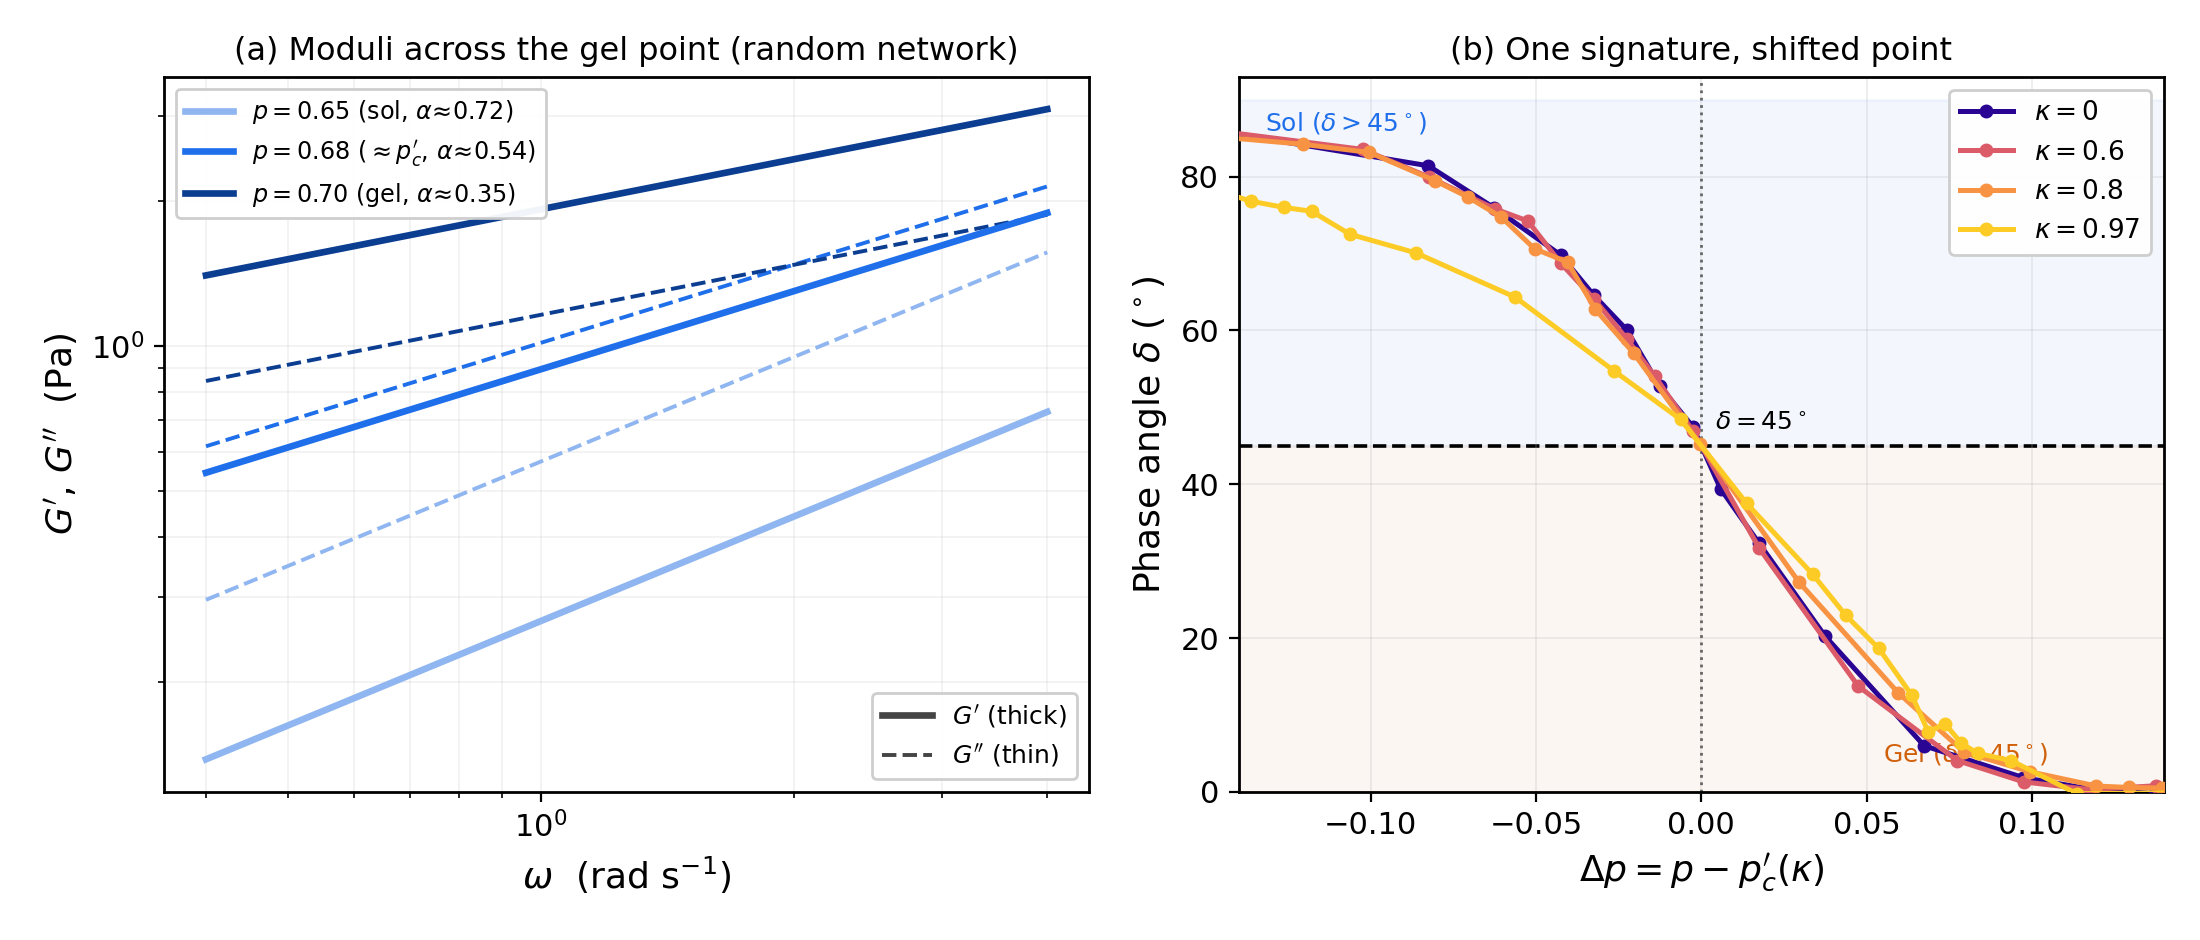
\includegraphics[width=0.9\linewidth]{fig3_gser_spectra.png}
  \caption{\textbf{One signature, shifted point.}
    (a) GSER-derived $G'(\omega)$, $G''(\omega)$ for the random ($\kap=0$) network at occupation
    densities straddling $\pcp$: viscous ($G''>G'$) below, elastic ($G'>G''$) above, and
    $G'\approx G''$ ($\delta\approx45^{\circ}$) at the gel point---the Winter--Chambon signature.
    (b) Phase angle $\delta=90\alpha$ versus distance from the gel point $\Delta p=p-\pcp(\kap)$
    for several $\kap$; all collapse through $\delta=45^{\circ}$ at $\Delta p=0$---the same critical
    rheology at each $\kap$'s own (shifted) gel point.}
  \label{fig:gser}
\end{figure}

\bibliographystyle{apsrev4-2}
\bibliography{references_enhanced}

\end{document}
